\chapter{人类演化概览}\label{ch:g12:human-evolution}

在一层距今三百五十万年的火山灰中，两
道脚印并排延伸了 27 米。它们
是直立行走的生物留下的，足跟先着地，足弓明显，
大脚趾与其余脚趾排成一线——这样的足与我们的相似——那时
世上还没有脑比猿大的生物。直立行走
出现得早了两百万年；脑、工具与语言
则出现在后来，而且并非直线式演化，而是沿着一丛\omterm{def:g10:biodiversity-scales:species}{物种}的分支展开，其中大多数
没有留下后代。本章将前两章的工具
——共有性状、树、年代和 \omterm{def:g10:universal-dna:information}{DNA}——应用于通向我们的
谱系。

\section{灵长类中的人类}

\begin{proposition}[人类在树中的位置]\label{prop:g12:human-evolution:place}
人类是灵长类：哺乳动物，手能抓握，指甲取代了爪，
眼睛朝前，相对体型而言脑较大。在灵长类之内，
大猿——红毛猩猩、大猩猩、黑猩猩、倭黑猩猩、
人——构成一个\omterm{prop:g12:phylogenetic-trees:rules}{演化支}，其中黑猩猩与倭黑猩猩
是人类的姐妹类群：我们的 \omterm{def:g10:universal-dna:information}{DNA} 与它们的在约
1.2\% 的位点上存在差异，两条谱系的共同祖先生活在
约六到七百万年前的非洲。该祖先既不是
黑猩猩，也不是人类；此后两条谱系都已各自演化。
\end{proposition}
\begin{proof}[证据]
性状矩阵与 \omterm{def:g10:universal-dna:information}{DNA} 比较（
见\cref{ch:g12:phylogenetic-trees}）表明：每个被测序的\omterm{def:g10:universal-dna:gene}{基因}都显示黑猩猩
与人的亲缘比与大猩猩更近；人类
2 号\omterm{def:g11:cell-cycle-mitosis:chromosome}{染色体}由两条\omterm{def:g11:cell-cycle-mitosis:chromosome}{染色体}首尾相接融合而成，这两条\omterm{def:g11:cell-cycle-mitosis:chromosome}{染色体}
在黑猩猩中仍保持分开——因此人类有 23 对，而黑猩猩有 24 对。
分子钟以较早灵长类分化的化石年代为校准，
由此给出人类与黑猩猩之间节点的年代。
\end{proof}

\begin{definition}[人类谱系]\label{def:g12:human-evolution:lineage}
称\emph{人类谱系}\index{人类谱系}为一个\omterm{prop:g12:phylogenetic-trees:rules}{演化支}，
即与现代人的亲缘比与黑猩猩更近的所有\omterm{def:g10:biodiversity-scales:species}{物种}：
由六百万年前节点的人类一侧所衍生的全部\omterm{def:g10:biodiversity-scales:species}{物种}。它
包括一个现存\omterm{def:g10:biodiversity-scales:species}{物种}\emph{Homo sapiens}，以及二十余个
化石\omterm{def:g10:biodiversity-scales:species}{物种}，包括南方古猿以及人属的若干
\omterm{def:g10:biodiversity-scales:species}{物种}（\emph{Homo}）。化石若显示出该谱系的衍生性状，即可归入其中：
直立行走、面部缩短、犬齿
变小，以及后来的大脑增大和工具。
\end{definition}

\section{谱系的性状}

\begin{proposition}[双足行走最先出现]\label{prop:g12:human-evolution:bipedalism}
\omterm{def:g12:human-evolution:lineage}{人类谱系}最早出现的衍生性状是习惯性
双足行走。这一点体现在骨骼上：颅底的开口
即脊髓穿过的孔，位于颅骨下方
而非后方，头部因此平衡于竖直的脊柱之上；
脊柱具双重弯曲；骨盆短而呈碗状；
股骨向内倾斜至膝部，使双脚位于身体的
重心之下；足部有足弓，大脚趾与其余脚趾排成一线，
适于蹬地，而非抓握。这些特征均已具备，
仅夹杂少量类猿特征，见于四百万年前的化石，其脑
容量不比黑猩猩的大。
\end{proposition}
\begin{proof}[证据]
火山灰中的脚印，距今 360 万年，显示出
跨步式步态，足跟先着地，足弓明显。一具
雌性南方古猿的骨骼，距今 320 万年、完整度为 40\%，具有
类人的骨盆与膝部，脑容量约 \qty{400}{cm^3}。同龄的
颅底中脊髓开口朝前，位于
颅骨之下。这些性状出现的顺序是：先为行走，超过
一百万年后才是脑的增长。
\end{proof}

\begin{omfigure}
\begin{tikzpicture}
  \node[anchor=south west, inner sep=0] (img) at (0,0)
    {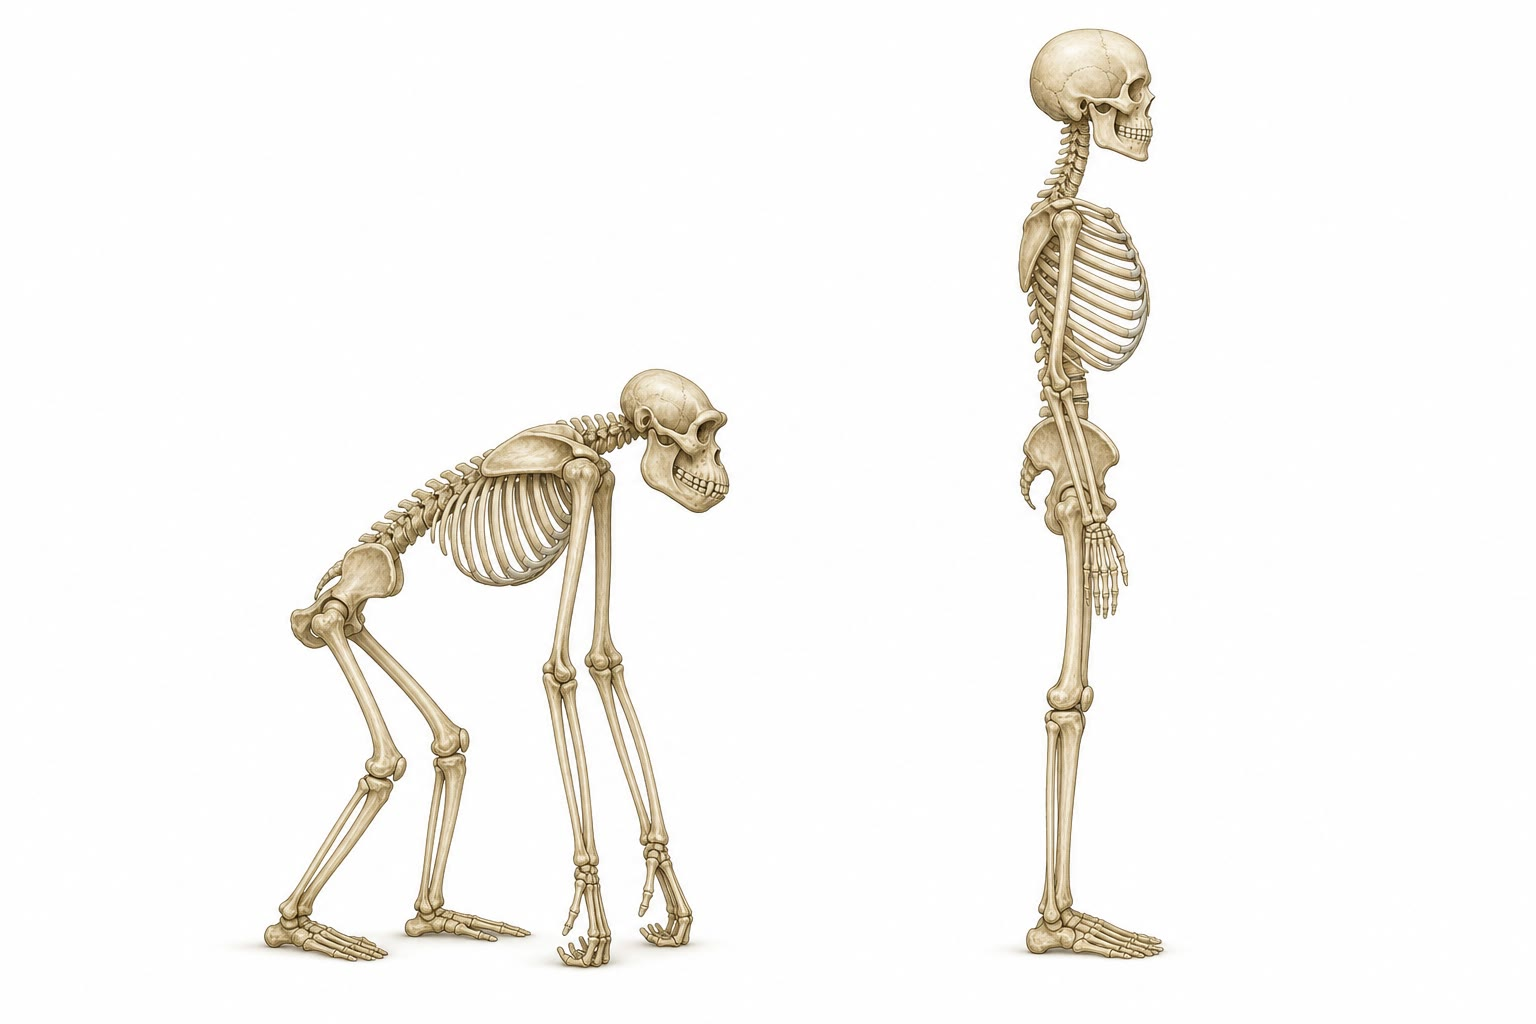
\includegraphics[width=0.56\linewidth]{images/book2/ai/fig-posture-skeletons.jpg}};
  \begin{scope}[x={(img.south east)}, y={(img.north west)},
      every node/.style={font=\scriptsize}]
    \draw[omDef, thick] (0.42,0.585) -- (0.42,0.98) node[above, align=center] {黑猩猩：枕骨大孔 \\ 位于颅骨后方};
    \draw[omDef, thick] (0.29,0.50) -- (-0.03,0.62) node[left, align=right] {斜向脊柱，\\ 头部前倾};
    \draw[omDef, thick] (0.23,0.42) -- (-0.03,0.40) node[left] {狭长的骨盆};
    \draw[omDef, thick] (0.25,0.26) -- (-0.03,0.18) node[left] {髋与膝弯曲};
    \draw[omDef, thick] (0.70,0.86) -- (1.03,0.90) node[right, align=left] {人类：枕骨大孔 \\ 位于颅骨下方};
    \draw[omDef, thick] (0.68,0.71) -- (1.03,0.68) node[right, align=left] {竖直脊柱 \\ 具双重弯曲};
    \draw[omDef, thick] (0.70,0.54) -- (1.03,0.48) node[right] {短而呈碗状的骨盆};
    \draw[omDef, thick] (0.69,0.32) -- (1.03,0.26) node[right] {膝位于躯干之下};
  \end{scope}
\end{tikzpicture}

{\small 黑猩猩与人类骨骼的侧视图。猿类中
脊髓从颅骨后方穿出，头部
自斜向脊柱前倾悬垂，髋与膝弯曲；双足行走者中，
颅底开口位于颅骨下方，头部平衡于竖直脊柱
之上，脊柱具双重弯曲，骨盆短而呈碗状，膝位于
躯干之下。化石的颅底、骨盆或膝部可用来
判断其步态。}
\end{omfigure}

\begin{omfigure}
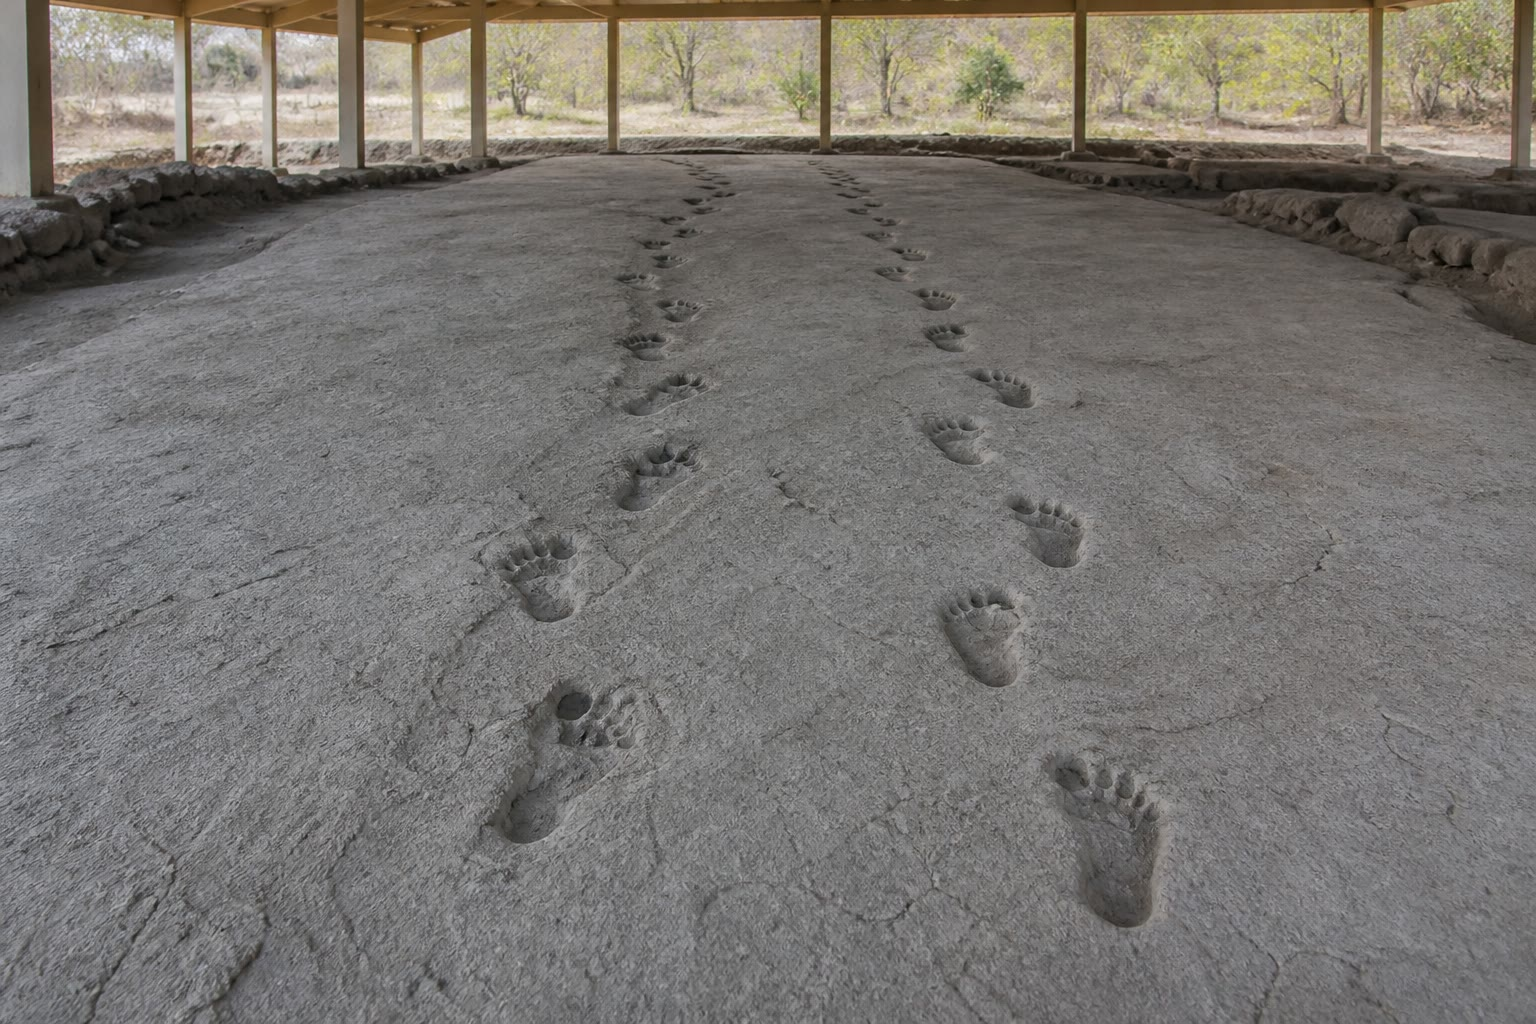
\includegraphics[width=0.6\linewidth]{images/book2/ai/g12-human-footprints.jpg}

{\small 保存于硬化火山灰中的一串脚印。足跟
先着地，足弓明显，大脚趾排成一线：直立行走者留下的
脚印，比最早的石器早数百万年。}
\end{omfigure}

\begin{proposition}[随后是大脑、工具与面部]\label{prop:g12:human-evolution:brain}
约 250 万年前起，谱系显示出第二组
衍生性状：脑容量由 \qty{450}{cm^3} 增至
\qty{1350}{cm^3}，面部与颌骨位于其下方并缩小，出现下巴，以及
石器——先是打出刃口的砾石，然后是修成形的手斧，
再后是石片、尖状器和带柄的复合工具。距今一百万年前已能控制用火，
距今十万年前已有埋葬死者的做法，距今四万年前出现
绘画图像。脑与工具共同发展，彼此
互相促进，历时两百多万年。
\end{proposition}
\admitted

\begin{omfigure}
\begin{tikzpicture}
\begin{axis}[
  width=0.9\linewidth, height=6cm,
  axis x line=bottom, axis y line=left,
  x dir=reverse, xmin=0, xmax=4.2, ymin=300, ymax=1600,
  xlabel={百万年前}, ylabel={脑容量（$\mathrm{cm^3}$）},
  xlabel style={font=\small, at={(axis description cs:0.5,-0.12)}, anchor=north},
  ylabel style={font=\small},
  tick label style={font=\small}, xtick={4,3,2,1,0}, ytick={400,800,1200,1600},
  clip=false,
]
\addplot[only marks, mark=*, mark size=2.2pt, omThm] coordinates
  {(3.5,420) (2.5,450) (2.0,600) (1.5,850) (0.8,1000) (0.4,1250) (0.1,1450) (0.05,1350)};
\node[font=\scriptsize, anchor=south] at (axis cs:3.5,450) {南方古猿};
\node[font=\scriptsize, anchor=north] at (axis cs:2.0,570) {能人 \emph{H. habilis}};
\node[font=\scriptsize, anchor=south] at (axis cs:1.5,880) {早期 \emph{H. erectus}};
\node[font=\scriptsize, anchor=north] at (axis cs:0.8,970) {晚期 \emph{H. erectus}};
\node[font=\scriptsize, anchor=south] at (axis cs:0.5,1280) {海德堡人 \emph{H. heidelbergensis}};
\node[font=\scriptsize, anchor=east] at (axis cs:0.12,1470) {尼安德特人};
\node[font=\scriptsize, anchor=north] at (axis cs:0.05,1320) {现代人 \emph{H. sapiens}};
\draw[dashed, gray] (axis cs:4.2,400) -- (axis cs:0,400);
\node[font=\scriptsize, gray, anchor=south east] at (axis cs:0.05,405) {黑猩猩（现今）};
\end{axis}
\end{tikzpicture}

{\small \omterm{def:g12:human-evolution:lineage}{人类谱系}各\omterm{def:g10:biodiversity-scales:species}{物种}的脑容量随年代的变化（取近似平均值）。
直立行走的最初两百万年间，脑容量与猿类相当，保持在 \qty{400}{cm^3} 左右；
此后两百万年间，脑容量增至约三倍；
尼安德特人的脑略大于现代人的脑。}
\end{omfigure}

\begin{omfigure}
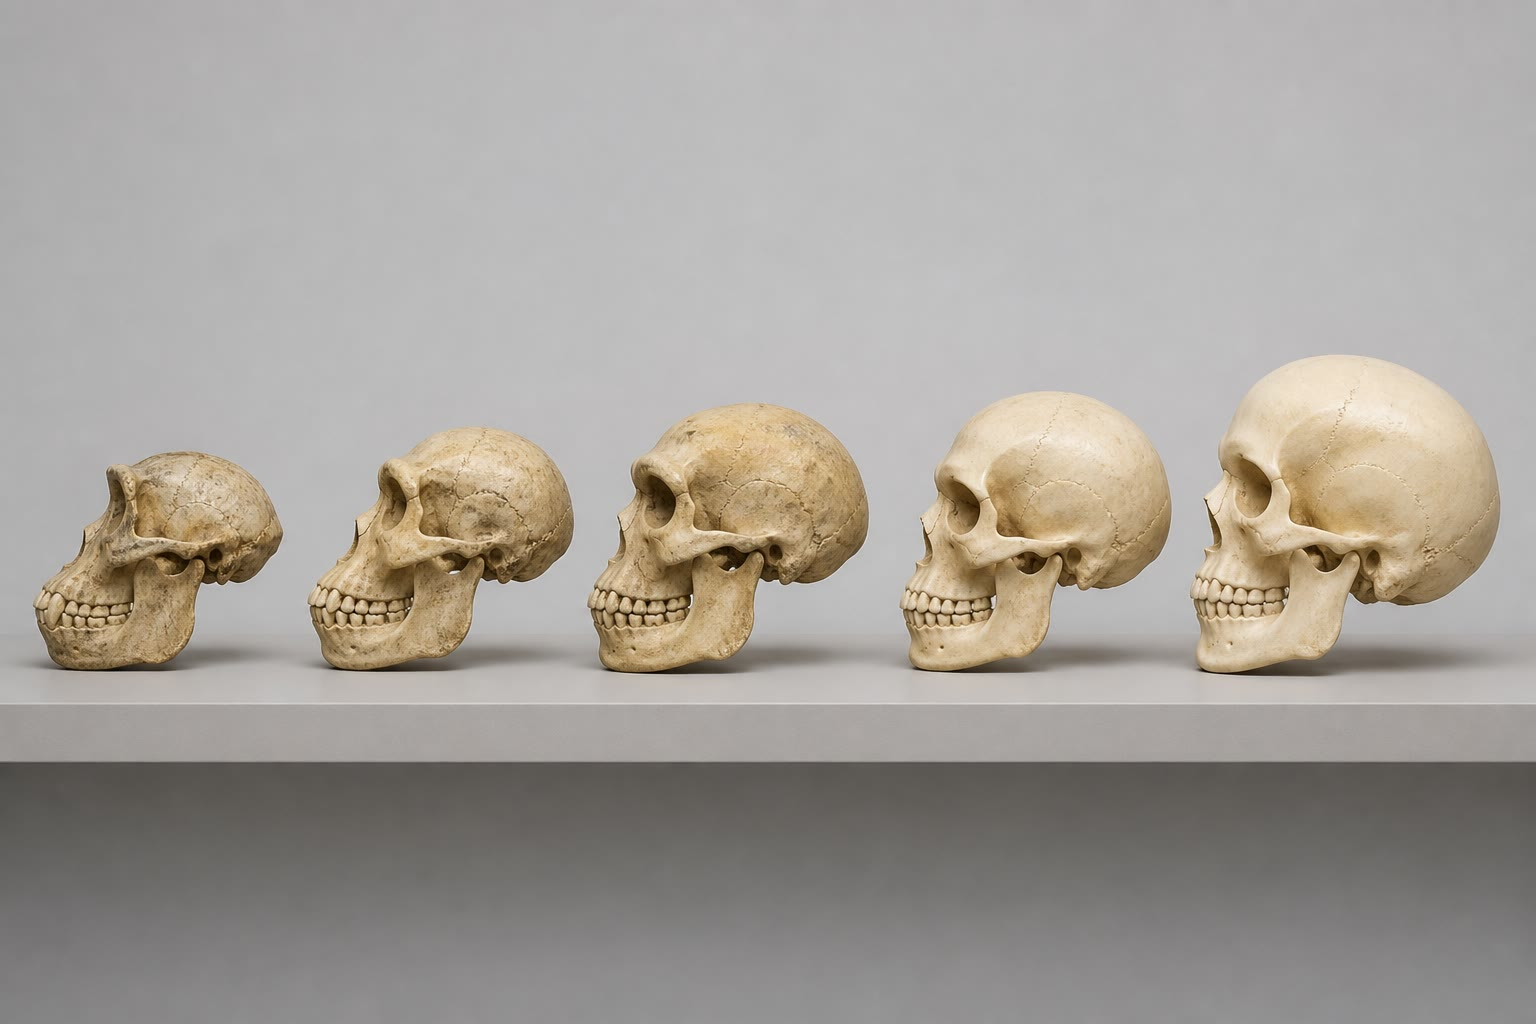
\includegraphics[width=0.66\linewidth]{images/book2/ai/g12-human-skulls.jpg}

{\small \omterm{def:g12:human-evolution:lineage}{人类谱系}各\omterm{def:g10:biodiversity-scales:species}{物种}的头骨侧视图，自南方古猿至现代人：
脑颅逐渐膨大，面部退缩于其下，
眉脊渐趋平缓，并出现下巴。}
\end{omfigure}

\begin{example}[读懂头骨]\label{ex:g12:human-evolution:skull}
一具化石头骨，底部有脊柱孔，脑颅容量为
\qty{450}{cm^3}，颌骨粗大，面部前突，属南方古猿：能直立行走，脑量小。
脑容量为 \qty{900}{cm^3}，眉脊粗重、额部后倾且无下巴者，
是 \emph{Homo
erectus}。脑容量为 \qty{1400}{cm^3}，额部高，面部小而收于脑颅之下，并有下巴者，
是现代人。谱系树上这些性状的排列次序，
即其在岩层中出现的先后，
也就是岩层所记录的时间顺序。
\end{example}

\section{灌木，而非阶梯}

\begin{proposition}[多个物种同时存在]\label{prop:g12:human-evolution:bush}
\omterm{def:g12:human-evolution:lineage}{人类谱系}并非一条由祖先与后代相接的单线，
而是一丛\omterm{def:g10:biodiversity-scales:species}{物种}，
其中若干\omterm{def:g10:biodiversity-scales:species}{物种}曾同时生存：二百万年前，两三种南方古猿与最早的 \emph{Homo} 并存；
\emph{Homo erectus} 遍布三大洲，
与此同时，非洲又出现了其他\omterm{def:g10:biodiversity-scales:species}{物种}；直到距今仅五万年前，
现代人仍与欧洲的尼安德特人、亚洲的另一\omterm{def:g12:selection-drift-speciation:population}{种群}、
以及一个体型较小、生活在岛上的\omterm{def:g10:biodiversity-scales:species}{物种}共享地球。
这丛灌木的大多数分支以灭绝告终，
唯有我们这一支留存至今。
\end{proposition}
\begin{proof}[证据]
不同\omterm{def:g10:biodiversity-scales:species}{物种}的化石见于同一遗址、同一年代的地层中。
尼安德特人与现代人的遗骸在欧洲重叠共存了数千年。
从尼安德特人和亚洲\omterm{def:g12:selection-drift-speciation:population}{种群}的骨骼中提取的 \omterm{def:g10:universal-dna:information}{DNA}，与我们的不同，
却又存在于我们体内：
非洲以外的人群携带约 2\% 的尼安德特人 \omterm{def:g10:universal-dna:information}{DNA}，
部分太平洋人群则携带数个百分点的亚洲\omterm{def:g12:selection-drift-speciation:population}{种群} \omterm{def:g10:universal-dna:information}{DNA}，
这是两者相遇时杂交留下的痕迹。
谱系的分支在消亡之前已彼此接触。
\end{proof}

\begin{omfigure}
\begin{tikzpicture}[font=\small]
  \tikzset{bar/.style={line width=6pt, line cap=butt}}
  % time axis: 0 at right, 4 Ma at left; 3 cm per Ma
  \draw[->, thick] (0,-0.4) -- (12.6,-0.4);
  \foreach \t/\l in {0/{4}, 3/{3}, 6/{2}, 9/{1}, 12/{0}} { \draw (\t,-0.3) -- (\t,-0.5); \node[anchor=north, font=\scriptsize] at (\t,-0.55) {\l}; }
  \node[anchor=north, font=\scriptsize] at (6.3,-0.95) {百万年前};
  % species bars: (start, end) in Ma -> x = (4 - Ma)*3
  \draw[bar, omDef!60] (0.3,0.4) -- (3.3,0.4); \node[anchor=west, font=\scriptsize] at (3.4,0.4) {南方古猿阿法种 \emph{Australopithecus afarensis}};
  \draw[bar, omDef!60] (2.1,1.0) -- (5.7,1.0); \node[anchor=west, font=\scriptsize] at (5.8,1.0) {南方古猿非洲种 \emph{A. africanus}};
  \draw[bar, omDef!40] (3.9,1.6) -- (8.4,1.6); \node[anchor=west, font=\scriptsize] at (8.5,1.6) {傍人 \emph{Paranthropus}};
  \draw[bar, omProp!60] (4.8,2.2) -- (7.8,2.2); \node[anchor=west, font=\scriptsize] at (7.9,2.2) {能人 \emph{Homo habilis}};
  \draw[bar, omProp!60] (6.3,2.8) -- (11.7,2.8); \node[anchor=west, font=\scriptsize] at (11.8,2.8) {直立人 \emph{H. erectus}};
  \draw[bar, omThm!50] (9.9,3.4) -- (11.4,3.4); \node[anchor=east, font=\scriptsize] at (9.8,3.4) {海德堡人 \emph{H. heidelbergensis}};
  \draw[bar, omThm!50] (10.8,4.0) -- (11.88,4.0); \node[anchor=east, font=\scriptsize] at (10.7,4.0) {尼安德特人};
  \draw[bar, omMeth!70] (11.1,4.6) -- (12.0,4.6); \node[anchor=east, font=\scriptsize] at (11.0,4.6) {现代人 \emph{H. sapiens}};
\end{tikzpicture}

{\small \omterm{def:g12:human-evolution:lineage}{人类谱系}的部分\omterm{def:g10:biodiversity-scales:species}{物种}及其化石所属的时期。
几乎在任一时间点，都有数个\omterm{def:g10:biodiversity-scales:species}{物种}并存，
该谱系犹如一丛灌木，仅有一根枝条留存至今。}
\end{omfigure}

\begin{proposition}[现代人]\label{prop:g12:human-evolution:sapiens}
\emph{Homo sapiens} 约于 300\,000 年前出现于非洲，
其颅骨高而圆，面部小，并有下巴，可借此识别。
约 60\,000 年前，小群体离开非洲，
在 50\,000 年内遍及除南极洲外的各大洲，
并与所遇到的较早\omterm{def:g12:selection-drift-speciation:population}{种群}相遇，部分地吸收了它们。所有现存的人类都源自该非洲\omterm{def:g12:selection-drift-speciation:population}{种群}：
整个\omterm{def:g10:biodiversity-scales:species}{物种}的\omterm{def:g10:biodiversity-scales:biodiversity}{遗传多样性}
小于非洲某一地区黑猩猩群体的\omterm{def:g10:biodiversity-scales:biodiversity}{遗传多样性}，
而且在非洲最为丰富，
并随离开非洲、沿扩散路线而逐步减少——
这正是相继奠基群体留下的印记。
\end{proposition}
\admitted

\begin{omfigure}
\begin{tikzpicture}
\begin{axis}[
  ybar, bar width=14pt,
  width=0.84\linewidth, height=5.2cm,
  axis x line=bottom, axis y line=left,
  ymin=0, ymax=6, ylabel={占基因组的\%},
  ylabel style={font=\small},
  symbolic x coords={sub-Saharan Africa, Europe, East Asia, Melanesia},
  xtick=data, xticklabels={撒哈拉以南非洲, 欧洲, 东亚, 美拉尼西亚}, tick label style={font=\small},
  enlarge x limits=0.2, ytick={0,2,4,6},
  legend style={at={(0.03,0.95)}, anchor=north west, font=\small, draw=none},
]
\addplot[fill=omThm!50, draw=omThm] coordinates {(sub-Saharan Africa,0.1) (Europe,1.8) (East Asia,2.2) (Melanesia,2.0)};
\addplot[fill=omDef!50, draw=omDef] coordinates {(sub-Saharan Africa,0) (Europe,0) (East Asia,0.2) (Melanesia,3.5)};
\legend{尼安德特人 DNA, 亚洲人群的 DNA}
\end{axis}
\end{tikzpicture}

{\small 从两个已灭绝\omterm{def:g12:selection-drift-speciation:population}{种群}继承的\omterm{def:g10:universal-dna:gene}{基因}组份额，
按地区（已取整）。走出非洲的\omterm{def:g12:selection-drift-speciation:population}{种群}与尼安德特人相遇并杂交，
抵达西太平洋的\omterm{def:g12:selection-drift-speciation:population}{种群}还与亚洲人群相遇；
灌木状谱系的各分支曾相互交换\omterm{def:g10:universal-dna:gene}{基因}，
直至只余一支，其余全部终止。}
\end{omfigure}

\section{是什么造就了我们}

\begin{proposition}[先是基因，然后是文化]\label{prop:g12:human-evolution:culture}
谱系的性状按前几章所述产生：
\omterm{def:g11:mutations:mutation}{突变}，包括\omterm{prop:g12:diversification-of-life:development}{发育基因}调控的改变
（大脑生长延长，面部缩短），在非洲稀树草原的环境中经\omterm{def:g12:selection-drift-speciation:selection}{自然选择}保留，
也可在小\omterm{def:g12:selection-drift-speciation:population}{种群}中因\omterm{prop:g12:selection-drift-speciation:drift}{遗传漂变}而保留。
但谱系又增加了第二种遗传方式——
即\cref{ch:g12:diversification-of-life}中所述的行为传递，
其规模远超其他任何\omterm{def:g10:biodiversity-scales:species}{物种}：工具、用火、语言、
合作与教学。文化在一生之内积累，并
传给所有学习它的人，而不仅限于后代；过去十万
年间，对人类影响最大的变化都是文化性的，
而该\omterm{def:g10:biodiversity-scales:species}{物种}演化于其中的环境，很大程度上是
它自己所造就的。
\end{proposition}
\admitted

\begin{method}[化石的定位]\label{met:g12:human-evolution:placing}
\begin{enumerate}
  \item 确定地层年代（火山矿物的放射性衰变，或
        地层的已知年龄）。
  \item 判断步态：脊柱开口的位置、骨盆与股骨的形状，
        以及足部。
  \item 测量脑颅；记录面部、眉脊、
        下巴和牙齿。
  \item 列出存在与缺失的衍生状态，并将
        化石依\cref{ch:g12:phylogenetic-trees}中的规则放在树上：
        若其性状组合与某节点相符，则作为该节点附近的侧枝，
        而非“祖先”。
  \item 若骨骼保存得足够好，则读取 \omterm{def:g10:universal-dna:information}{DNA}，并与
        现生\omterm{def:g12:selection-drift-speciation:population}{种群}作比较。
\end{enumerate}
\end{method}

\begin{remark}[并不存在“缺失的环节”]\label{rem:g12:human-evolution:link}
该说法假设链条上只有一处缺口；化石记录实为一丛灌木，
分支众多，多数仅由少数骨骼得知。而“环节”
介于我们与黑猩猩之间者，是一个节点——一个已灭绝的\omterm{def:g12:selection-drift-speciation:population}{种群}，
既非人类，也非黑猩猩，而不是介于二者之间的生物。化石所显示的，
依岩层保存的先后顺序，所显示的是每一衍生性状
依次出现：先是足，然后是脑，再是工具，接着是
下巴——而在过去五万年间，则是一个\omterm{def:g10:biodiversity-scales:species}{物种}的产物，
其演化如今很大程度上由它自己所造就。
\end{remark}

\section{练习}

\begin{exercise}[$\star$]\label{exo:g12:human-evolution:1}
哪一现存\omterm{def:g10:biodiversity-scales:species}{物种}与人类亲缘关系最近，两谱系
约在多久以前分开？
\end{exercise}

\begin{exercise}[$\star$]\label{exo:g12:human-evolution:2}
列出直立行走的四种骨骼特征。
\end{exercise}

\begin{exercise}[$\star$]\label{exo:g12:human-evolution:3}
根据脑容量图，求出一个南方古猿、
早期 \emph{Homo erectus} 和一个现代人的脑容量。
\end{exercise}

\begin{exercise}[$\star$]\label{exo:g12:human-evolution:4}
为何\omterm{def:g12:human-evolution:lineage}{人类谱系}被描述为灌木状，而非梯子状？
\end{exercise}

\begin{exercise}[$\star$]\label{exo:g12:human-evolution:5}
\emph{Homo sapiens} 出现于何地、何时，以及
人类\omterm{def:g10:biodiversity-scales:biodiversity}{遗传多样性}的分布说明了什么？
\end{exercise}

\begin{exercise}[$\star\star$]\label{exo:g12:human-evolution:6}
人类的 2 号\omterm{def:g11:cell-cycle-mitosis:chromosome}{染色体}对应于两条黑猩猩\omterm{def:g11:cell-cycle-mitosis:chromosome}{染色体}，
两者首尾相接。试说明这如何解释二者\omterm{def:g11:cell-cycle-mitosis:chromosome}{染色体}数目的不同，
并说明为何它是亲缘关系的证据，而非
反对亲缘关系的证据。
\end{exercise}

\begin{exercise}[$\star\star$]\label{exo:g12:human-evolution:7}
在该谱系中，直立行走与大脑增大，哪一个先出现？
两者相差多长时间？请引用证据。
\end{exercise}

\begin{exercise}[$\star\star$]\label{exo:g12:human-evolution:8}
根据时间轴图，哪些\omterm{def:g10:biodiversity-scales:species}{物种}在两百万年前
曾共存？在 100\,000 年前又如何？
\end{exercise}

\begin{exercise}[$\star\star$]\label{exo:g12:human-evolution:9}
一位欧洲血统的人携带 2\% 的尼安德特人 \omterm{def:g10:universal-dna:information}{DNA}。请说明
这一比例记录的是何种事件，以及为何撒哈拉以南非洲人
几乎不携带此类 \omterm{def:g10:universal-dna:information}{DNA}。
\end{exercise}

\begin{exercise}[$\star\star$]\label{exo:g12:human-evolution:10}
运用\cref{met:g12:human-evolution:placing}分析一个
脊柱孔位置靠前、容积为 \qty{500}{cm^3}、颌骨粗大的颅骨，
发现于一个距今 2.8 百万年的地层中。
\end{exercise}

\begin{exercise}[$\star\star$]\label{exo:g12:human-evolution:11}
解释为何“人类源于猿类”可以被正确表述为“人类
即是猿类”，运用\omterm{prop:g12:phylogenetic-trees:rules}{演化支}的术语加以说明。
\end{exercise}

\begin{exercise}[$\star\star\star$]\label{exo:g12:human-evolution:12}
尼安德特人的脑略大于我们，并能制造精巧的工具，
然而在我们抵达欧洲后数千年内便消失，
提出两个与本章相符的假说，
并说明何种证据可以区分二者。
\end{exercise}

\begin{exercise}[$\star\star\star$]\label{exo:g12:human-evolution:13}
沿扩散路线，人类\omterm{def:g10:biodiversity-scales:biodiversity}{遗传多样性}随距非洲距离的增大而降低。
借助\cref{ch:g12:selection-drift-speciation}中的奠基者效应，
解释这一现象，并说明它表明
人类是如何扩散的。
\end{exercise}

\begin{exercise}[$\star\star\star$]\label{exo:g12:human-evolution:14}
乳糖耐受、高纬度地区的浅色皮肤以及对疟疾的抗性，
均是近一万年来演化出的人类性状。请说明
文化变迁（如乳制品生产、迁徙、农耕）如何产生
改变\omterm{def:g10:universal-dna:gene}{基因}的选择。
\end{exercise}

\begin{exercise}[$\star\star\star$]\label{exo:g12:human-evolution:15}
“人类的演化已经停止，因为医学与文化使我们免受
选择的影响。”请用一段话，结合\omterm{prop:g12:selection-drift-speciation:drift}{遗传漂变}，讨论上一题中的三种
性状，以及选择的含义。
\end{exercise}

\section{问题：灰烬中的行者}

\begin{problem}[{周末问题——通过两条足迹读取
步态、身高与速度；测量一排颅骨；并将一名在世学生的 DNA
追溯至三个种群}]
\label{pb:g12:human-evolution:1}
两条足迹，距今 3.6 百万年，平行延伸
\qty{27}{m}。足迹 A：脚印长 \qty{21.5}{cm}，步幅（
同一只脚相邻两印之间的距离）\qty{0.95}{m}。足迹 B：脚印长
\qty{18.5}{cm}，步幅 \qty{0.80}{m}。在现代人类中，脚长约占
站立身高的 15\%，而步行步幅约为身高的 0.8 倍，
对应于慢走。

\medskip
\noindent\textbf{第一部分——足迹。}
\begin{enumerate}
  \item 估算行者 A 与行者 B 的身高。
       \item 将每个步幅与身高的 0.8 倍进行比较，
        判断他们是在步行还是奔跑？
  \item 脚印显示出较深的足跟、足弓，以及与其他脚趾平行的
        大脚趾。这些特征分别说明足部与
        步态的什么？
  \item 直立行走的黑猩猩留下的脚印足底平坦、大脚趾外展，
        且无法长时间维持这一姿态。哪些
        \cref{prop:g12:human-evolution:bipedalism}中的特征
        可由这些足迹确定为其制造者所有，哪些
        尚不清楚？
  \item 同一时期最近的化石，脑容量为
        \qty{400}{cm^3}。这一组合（足如此，脑如彼）能确定
        该谱系性状出现的先后次序吗？
\end{enumerate}

\medskip
\noindent\textbf{第二部分——颅骨。}
五个颅骨的脑颅容积、年代与特征如下：
1：\qty{450}{cm^3}，3.0 百万年，面部突出，无颏。
2：\qty{650}{cm^3}，1.9 百万年，面部较小。
3：\qty{950}{cm^3}，1.0 百万年，眉弓粗壮，无颏。
4：\qty{1450}{cm^3}，60\,000 年，眉弓粗壮，无颏，
颅骨长而低。
5：\qty{1350}{cm^3}，30\,000 年，前额高，有颏。
\begin{enumerate}[resume]
  \item 将每个颅骨归入时间轴图中的一个类群。
  \item 绘制或描述五个颅骨的脑容量随年代的变化。在
        哪一时间区间内脑容量增长最快？
  \item 颅骨 4 的容量大于颅骨 5。仅凭脑容量
        能否判定为现代人？哪些性状可以做到？
  \item 颅骨 4 与颅骨 5 的时代有重叠。本章
        对二者所代表\omterm{def:g12:selection-drift-speciation:population}{种群}间的关系有何说法，
        以及哪些证据支持这一说法？
  \item 颅骨 1 与第一部分的足迹可能属于同一\omterm{def:g10:biodiversity-scales:species}{物种}。
        试说明该\omterm{def:g10:biodiversity-scales:species}{物种}为何应视为类祖先的
        \emph{近缘种}，而非已被证实的祖先，
        运用\cref{ch:g12:phylogenetic-trees}中的术语加以说明。
\end{enumerate}

\medskip
\noindent\textbf{第三部分——学生的\omterm{def:g10:universal-dna:gene}{基因}组。}
一名具有欧洲与美拉尼西亚血统的学生，其\omterm{def:g10:universal-dna:gene}{基因}组与
尼安德特人及已灭绝亚洲\omterm{def:g12:selection-drift-speciation:population}{种群}的\omterm{def:g10:universal-dna:gene}{基因}组作了比较：1.6\% 与尼安德特人\omterm{def:g10:universal-dna:gene}{基因}组相符，
1.8\% 与亚洲\omterm{def:g12:selection-drift-speciation:population}{种群}相符。
\begin{enumerate}[resume]
  \item 说明 1.6\% 的匹配率意味着什么，它记录了何种事件。
  \item 将她的数据与图表相比较。她的祖先\omterm{def:g12:selection-drift-speciation:population}{种群}中，
        哪些分别贡献了各部分的\omterm{def:g10:universal-dna:gene}{基因}？
  \item 若杂交发生于 50\,000 年前，且一代为
        25 年，则她与该事件相隔多少代？
        为何这一份额并未被稀释至零？
  \item 两个谱系为她贡献了\omterm{def:g10:universal-dna:gene}{基因}，尽管它们
        被称为不同的\omterm{def:g10:biodiversity-scales:species}{物种}。这对当时
        \cref{ch:g12:selection-drift-speciation}中的\omterm{def:g10:biodiversity-scales:species}{物种}界限说明了什么？
  \item 她的\omterm{def:g10:cells-common-unit:organelle}{线粒体} \omterm{def:g10:universal-dna:information}{DNA} 属于现代人类型，与所有在世者
        一样。这说明杂交的方向或
        结局是什么？
\end{enumerate}

\medskip
\noindent\textbf{第四部分——时钟与系统树。}
\begin{enumerate}[resume]
  \item 人类与黑猩猩的 \omterm{def:g10:universal-dna:information}{DNA} 相差 1.2\%；灵长类的
        \cref{ch:g12:phylogenetic-trees}中的灵长类分子钟以每百万年 0.27\%
        的速率运行。推算共同祖先的年代。
  \item 已知最古老的\omterm{def:g12:human-evolution:lineage}{人类谱系}化石距今 6 至 7
        百万年。这与你推算的年代相符吗？
  \item 列出时间轴图中一百万年前仍然活的\omterm{def:g10:biodiversity-scales:species}{物种}，
        并说明其中有多少种有现存后代。
  \item 说明为何谱系的最近十万年
        用文化变迁描述比用
        本章的性状描述更为恰当。
  \item 给出结论：行者 A 的身高与步态，足、脑与颏
        出现的先后次序，以及该学生所携带\omterm{def:g10:universal-dna:gene}{基因}的
        已灭绝\omterm{def:g12:selection-drift-speciation:population}{种群}数目。
\end{enumerate}
\end{problem}
